\PassOptionsToPackage{unicode=true}{hyperref} % options for packages loaded elsewhere
\PassOptionsToPackage{hyphens}{url}
%
\documentclass[]{article}
\usepackage{lmodern}
\usepackage{setspace}
\setstretch{2}
\usepackage{amssymb,amsmath}
\usepackage{ifxetex,ifluatex}
\usepackage{fixltx2e} % provides \textsubscript
\ifnum 0\ifxetex 1\fi\ifluatex 1\fi=0 % if pdftex
  \usepackage[T1]{fontenc}
  \usepackage[utf8]{inputenc}
  \usepackage{textcomp} % provides euro and other symbols
\else % if luatex or xelatex
  \usepackage{unicode-math}
  \defaultfontfeatures{Ligatures=TeX,Scale=MatchLowercase}
\fi
% use upquote if available, for straight quotes in verbatim environments
\IfFileExists{upquote.sty}{\usepackage{upquote}}{}
% use microtype if available
\IfFileExists{microtype.sty}{%
\usepackage[]{microtype}
\UseMicrotypeSet[protrusion]{basicmath} % disable protrusion for tt fonts
}{}
\IfFileExists{parskip.sty}{%
\usepackage{parskip}
}{% else
\setlength{\parindent}{0pt}
\setlength{\parskip}{6pt plus 2pt minus 1pt}
}
\usepackage{hyperref}
\hypersetup{
            pdftitle={Physcraper: a python package for continual update of evolutionary estimates using the Open Tree of Life},
            pdfborder={0 0 0},
            breaklinks=true}
\urlstyle{same}  % don't use monospace font for urls
\usepackage[margin = 1in]{geometry}
\usepackage{longtable,booktabs}
% Fix footnotes in tables (requires footnote package)
\IfFileExists{footnote.sty}{\usepackage{footnote}\makesavenoteenv{longtable}}{}
\usepackage{graphicx,grffile}
\makeatletter
\def\maxwidth{\ifdim\Gin@nat@width>\linewidth\linewidth\else\Gin@nat@width\fi}
\def\maxheight{\ifdim\Gin@nat@height>\textheight\textheight\else\Gin@nat@height\fi}
\makeatother
% Scale images if necessary, so that they will not overflow the page
% margins by default, and it is still possible to overwrite the defaults
% using explicit options in \includegraphics[width, height, ...]{}
\setkeys{Gin}{width=\maxwidth,height=\maxheight,keepaspectratio}
\setlength{\emergencystretch}{3em}  % prevent overfull lines
\providecommand{\tightlist}{%
  \setlength{\itemsep}{0pt}\setlength{\parskip}{0pt}}
\setcounter{secnumdepth}{5}
% Redefines (sub)paragraphs to behave more like sections
\ifx\paragraph\undefined\else
\let\oldparagraph\paragraph
\renewcommand{\paragraph}[1]{\oldparagraph{#1}\mbox{}}
\fi
\ifx\subparagraph\undefined\else
\let\oldsubparagraph\subparagraph
\renewcommand{\subparagraph}[1]{\oldsubparagraph{#1}\mbox{}}
\fi

% set default figure placement to htbp
\makeatletter
\def\fps@figure{htbp}
\makeatother

\usepackage{color}
\usepackage{hyperref}
\usepackage{caption}
\usepackage{blindtext}
\usepackage{url}
\usepackage[left]{lineno}
\linenumbers

\title{Physcraper: a python package for continual update of evolutionary estimates using the Open Tree of Life}
\author{}
\date{\vspace{-2.5em}}

\begin{document}
\maketitle

\textbf{1. Luna L. Sanchez Reyes}

School of Natural Sciences, University of California, Merced

email: \href{mailto:sanchez.reyes.luna@gmail.com}{\nolinkurl{sanchez.reyes.luna@gmail.com}}

\textbf{2. Martha Kandziora}

School of Natural Sciences, University of California, Merced

Department of Botany, Faculty of Science, Charles University, Prague, Czech Republic

email: \href{mailto:kandziom@natur.cuni.cz}{\nolinkurl{kandziom@natur.cuni.cz}}

\textbf{3. Emily Jane McTavish}

School of Natural Sciences, University of California, Merced

email: \href{mailto:ejmctavish@gmail.com}{\nolinkurl{ejmctavish@gmail.com}}

\textbf{Correspondence address}: Science and Engineering Building 1, University of California, Merced, 5200 N. Lake Rd, Merced CA 95343

\textbf{Correspondence email}: \href{mailto:sanchez.reyes.luna@gmail.com}{\nolinkurl{sanchez.reyes.luna@gmail.com}}, \href{mailto:ejmctavish@gmail.com}{\nolinkurl{ejmctavish@gmail.com}}

\textbf{Running title}: Continually updated gene trees with Physcraper

\textbf{Word count}: 3784

\textbf{Manuscript prepared for submission to Methods in Ecology and Evolution}

\textbf{Article type}: Application

\newpage

\begingroup\Large

\textbf{Abstract}
\endgroup

\begin{enumerate}
\def\labelenumi{\arabic{enumi}.}
\item
  Phylogenies are a key part of research in many areas of biology. Tools that automate
  some parts of the process of phylogenetic reconstruction, mainly molecular character matrix assembly,
  have been developed for the advantage of both specialists in the field of phylogenetics and nonspecialists.
  However, interpretation of results, comparison with previously available phylogenetic
  hypotheses, and choosing of one phylogeny for downstream analyses and discussion still impose difficulties
  to one that is not a specialist either on phylogenetic methods or on a particular group of study.
\item
  Physcraper is a command-line Python program that automates the update of published
  phylogenies by enriching underlying gene alignments with public DNA sequence data. It builds upon tools from the Open Tree of Life project to link taxonomic information across databases, providing a framework for straightforward comparison of published phylogenies with their updated versions.
\item
  Physcraper can be used by the nonspecialist, as a tool to generate phylogenetic
  hypotheses based on publicly available expert phylogenetic knowledge.
  Phylogeneticists and group specialists will find it useful as a tool to facilitate molecular dataset gathering and comparison
  of alternative phylogenetic hypotheses (topologies).
\item
  We hope that the Physcraper workflow demonstrates the benefits of doing open science for phylogenetics, encouraging more researchers to strive for better sharing practices. Physcraper can be used with any OS and is released under an open-source license. Detailed instructions for installation and
  use are available at \href{https://physcraper.readthedocs.io/en/tutorial/index.html}{https://physcraper.readthedocs}.
\end{enumerate}

\textbf{Keywords}: gene tree, interoperability, open science, open tree of life, phylogeny, public database, python, reproducibility, taxonomy, updated alignment

\newpage

\hypertarget{introduction}{%
\section{Introduction}\label{introduction}}

Phylogenetic estimates of evolutionary relationships capture the shared history of living organisms, and provide key context for all our biological observations.
Public biological databases constitute an amazing resource for evolutionary estimation, but a large portion of molecular data publicly available has never been incorporated into any phylogenetic estimate. Extending existing phylogenetic estimates with new DNA sequence data, geographical location, and other metadata in a reproducible and continuous manner is possible by automating connections between biological databases. Here, we introduce Physcraper, a tool that uses existing phylogenetic research from public biological databases to update a starting tree and single locus alignments, to build upon molecular data that taxon specialists have assessed and deemed appropriate for a specific phylogenetic scope.

The prevalence of taxonomic idiosyncrasies across databases represent a key challenge to automatically connecting data from disparate biological databases in a phylogenetic context. To standardize taxonomic names, a unified system is needed. The main aim of the Open Tree of Life (OpenTree from now on) project
is to construct a comprehensive, dynamic and digitally-available tree of life by synthesizing published phylogenetic trees along with taxonomic data. Currently, OpenTree's ``synthetic'' tree comprises 2.3 million tips, of which around 90,000 are represented by phylogenetic estimates - the remaining 1.4 million taxa are placed in the tree based on their taxonomic assignment. To achieve this, OpenTree unifies taxonomy from various databases (Rees \& Cranston \protect\hyperlink{ref-rees2017automated}{2017}) such as the USA National Center for Biodiversity Information (NCBI) molecular database GenBank (Benson \emph{et al.} \protect\hyperlink{ref-benson2000genbank}{2000}; Wheeler \emph{et al.} \protect\hyperlink{ref-wheeler2000database}{2000}), the Global Biodiversity Information Facility (GBIF; Secretariat \protect\hyperlink{ref-secretariat2017gbif}{2017}), and the World Register of Marine Species {[}WoRMS; www.marinespecies.org/{]}, providing a key resource that can be used to connect data from virtually any biological database to phylogenetic data that has been standardized to OpenTree's unified taxonomy.

Another challenge to incorporating molecular data from public databases to update phylogenetic knowledge is assembling high-quality homology hypotheses.
Species tree reconstructions from multiple single locus data sets taking into account the multispecies coalescent model are seen as the gold standard for inferring species relationships (Song \emph{et al.} \protect\hyperlink{ref-song2012resolving}{2012}).
Genomics has, and will continue to, revolutionize phylogenetic inference.
Yet, different research questions call for different genomic sequencing approaches, from whole genomes, to transcriptomes, restriction-site associated DNA sequencing, single nucleotide polymorphisms, microsatellites, and ultra-conserved elements, which has lead to largely non-overlapping genomic data sets across taxa, difficulting wide scale phylogenetic reconstructions.
While phylogenomics ameliorates the problem of non-overlapping genomic data sets by focusing on targeted capture of informative characters from independent and single-copy genetic markers (Jones \& Good \protect\hyperlink{ref-jones2016targeted}{2016}; Andermann \emph{et al.} \protect\hyperlink{ref-andermann2020guide}{2020}), decades of single locus sequencing have already generated homologous DNA data sets that can be used for phylogenetic reconstruction at many scales.

Indeed, more than a decade ago, GenBank release number 159 (April 15, 2007) already hosted 72 million non-genomic DNA sequences. These sequences were gauged to have the potential to resolve phylogenetic relationships of most (98.05\%) of the almost 241, 000 distinct taxa in the NCBI taxonomy at the time (Sanderson \emph{et al.} \protect\hyperlink{ref-sanderson2008phylota}{2008}). Assembling a DNA alignment from such a massive database can be done ``by hand'', but it requires huge amounts of time and it is mostly a non-reproducible approach. Computational pipelines that make DNA sequence search faster and more efficient, as well as more reproducible, have been applied to study evolutionary relationships among a variety of organisms (e.g., Smith \emph{et al.} \protect\hyperlink{ref-smith2009mega}{2009}; Izquierdo-Carrasco \emph{et al.} \protect\hyperlink{ref-izquierdo2014pumper}{2014}; Antonelli \emph{et al.} \protect\hyperlink{ref-antonelli2017toward}{2017}).
However, even during phylogenomic reconstructions, thoughtfully curated markers and alignments can improve phylogenetic reconstructions (Fragoso-Martínez \emph{et al.} \protect\hyperlink{ref-fragoso2017pilot}{2017}).

A way to incorporate the best of two worlds (massive amounts of newly released molecular data and fine-grained curation from human experts) is to rely on published manually curated homology hypotheses as ``jump-start'' alignments (Morrison \protect\hyperlink{ref-morrison2006multiple}{2006}). The TreeBASE database (Piel \emph{et al.} \protect\hyperlink{ref-piel2009treebase}{2009}) hosts about 8, 200 publicly accessible alignments, providing information on evolutionary relationships of around 100, 000 distinct taxa \href{https://www.treebase.org/treebase-web/home.html\#:~:text=TreeBASE\%20is\%20produced\%20and\%20governed,mapped\%20to\%20104\%2C593\%20distinct\%20taxa.}{(see TreeBASE's website about)}, representing a source of valuable expert knowledge. Linking published alignments with public molecular data that has not yet been included in any public phylogenetic estimate, has the potential to accelerate the enrichment and updating of phylogenetic relationships in many regions of the tree of life. The phylogenies associated to TreeBASE alignments have been integrated to the OpenTree's datastore, the Phylesystem (McTavish \emph{et al.} \protect\hyperlink{ref-mctavish2015phylesystem}{2015}), and metadata linking them to their corresponding alignment repository is available, providing a non-automated way of linking trees with the alignment that generated them.

Physcraper relies on programmatic access protocols to automatically link molecular data from GenBank to alignments from TreeBASE and phylogenies from OpenTree's Phylesystem, to continually update and enrich phylogenetic knowledge based on expertly-curated homology hypotheses. Physcraper also provides new types of access to various general OpenTree programmatic tools for comparison of existing phylogenetic hypotheses with newly generated ones.
Physcraper is coded as a Python pipeline that focuses on data interoperability, by integrating taxonomic name matching across biological databases. This integration also allows users to rapidly place new data from a diverse range of biological databases in an evolutionary context, making a variety of downstream analyses straightforward.

\hypertarget{the-physcraper-framework}{%
\section{The Physcraper framework}\label{the-physcraper-framework}}

\begin{figure}

{\centering 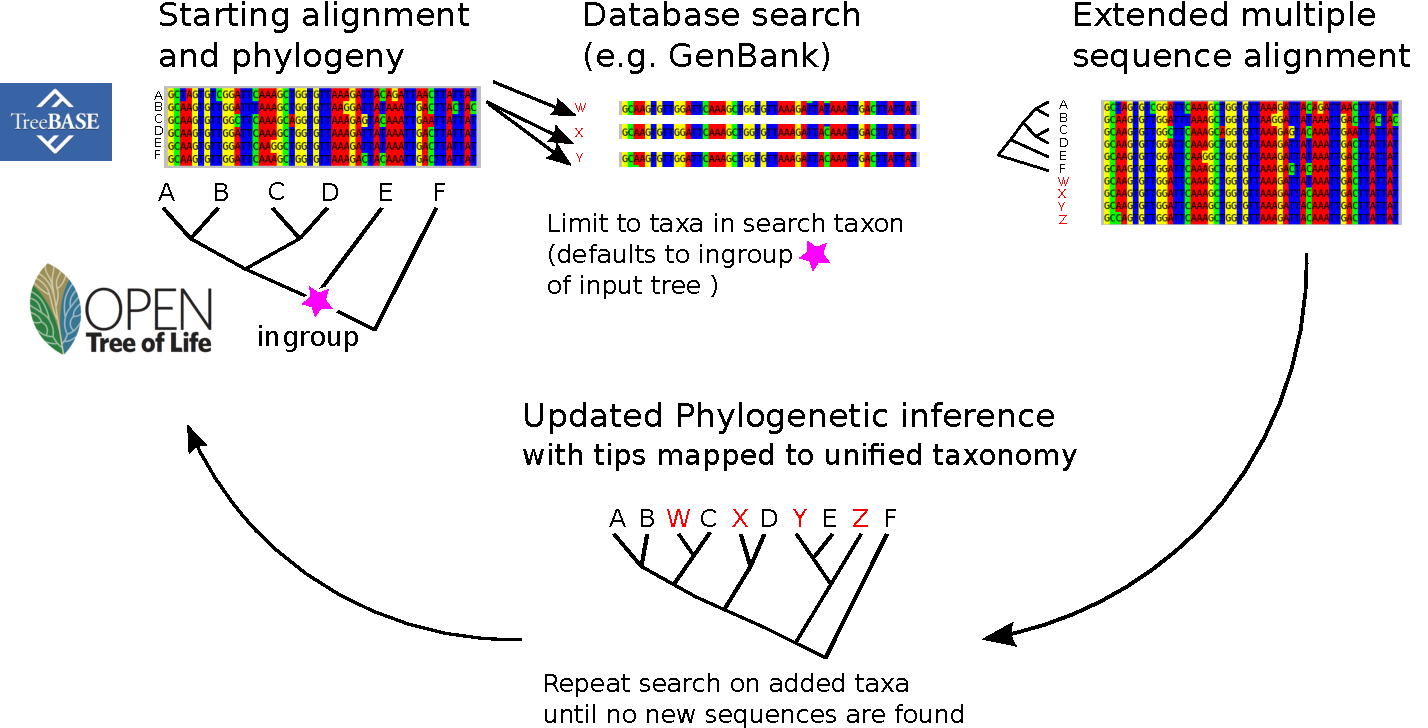
\includegraphics[width=0.85\linewidth]{docs/figs/schematic} 

}

\caption{The Physcraper framework consists of 4 steps (see text). The software is fully described on its documentation website at physcraper.readthedocs.io, along with installation instructions, function usage descriptions, examples and tutorials.}\label{fig:framework}
\end{figure}

The general Physcraper framework is depicted in Figure \ref{fig:framework}. Briefly, it consists of 4 steps: 1) identifying and processing a phylogenetic tree to update and its underlying alignment; 2) performing a constrained BLAST search of sequences from the original alignment on the GenBank DNA database, and filtering of newly found sequences; 3) profile-aligning new sequences that passed the filtering to the original alignment; 4) performing a phylogenetic analysis and comparing the updated tree to previous phylogenetic estimates in the focus group. Next, we will describe technical details for each step.

\hypertarget{the-inputs-a-tree-and-an-alignment}{%
\subsection{The inputs: a tree and an alignment}\label{the-inputs-a-tree-and-an-alignment}}

\begin{itemize}
\item
  In order to take advantage of the OpenTree tools, it is reccommended that the input tree is either stored in the
  OpenTree \href{https://github.com/opentreeoflife/phylesystem}{Phylesystem}, or submitted via OpenTree's curator \href{https://tree.opentreeoflife.org/curator}{application} (McTavish \emph{et al.} \protect\hyperlink{ref-mctavish2015phylesystem}{2015}).
  Currently, only trees connected to a published study can be stored in the Phylesystem.
  Users can choose from among the 2, 950 studies in OpenTree's Phylesystem that have alignments on TreeBASE.
  If the user is not ready to make the input tree public, tree tip labels must be first standardized to the unified OpenTree taxonomy using OpenTree's bulk Taxonomic Name Resolution Service \href{https://tree.opentreeoflife.org/curator/tnrs/}{TNRS} tool. \emph{Should we say that it is based on Boyle's 2012 algorithm? or is it a TNRS algorithm independently developed by the OpenTree team?}
  This step is referred to as taxonomic name mapping and Phylesystem stored trees are processed in this way upon submission.
  Physcraper saves a summary ``csv'' file with results from the taxon name standardization for advantage of the user.
  If taxon names can't be mapped, their taxonomic information can't be used in comparison analysis. They will still be used in the sequence search and phylogenetic reconstruction steps.
  Mapping tip names to OpenTree's unified taxonomy saves a set of user defined characteristics
  that are essential for automatizing the phylogeny updating process. The most relevant of these is the standardized taxonomic names and the definition of ingroup and outgroup taxa, allowing to automatically set the root for the updated tree on the final steps of the pipeline.
\item
  The input alignment should be a single locus alignment that was used to generate the tree. Alignments are often stored in a public repository such as TreeBase (Piel \emph{et al.} \protect\hyperlink{ref-piel2009treebase}{2009}; Vos \emph{et al.} \protect\hyperlink{ref-vos2012nexml}{2012}),
  DRYAD (\href{http://datadryad.org/}{www.datadryad.org}), or a data repository associated with the journal where the tree was originally published.
  If the alignment is stored in TreeBase, Physcraper downloads it directly,
  either from the TreeBASE website (\href{https://treebase.org/}{www.treebase.org})
  or through the TreeBASE GitHub repository (SuperTreeBASE; \href{https://github.com/TreeBASE/supertreebase}{github.com/TreeBASE/supertreebase}).
  If the alignment is on another repository, or constitutes personal data, a path to a local copy of the alignment has to be provided.
\item
  Single locus alignments sometimes have fewer taxa than the tree inferred from the full concatenated data, simply because a single molecular marker usually does not cover all the taxa sampled for the full phylogenetic analysis. Physcraper prunes the input tree to taxa found in the alignment, and verifies that all taxon names on the tips of the tree are in the DNA character matrix and vice versa. Technically, just one taxon name (and its corresponding sequence in the alignment) is needed to continue the algorithm. See next section.
\item
  The standardized and pruned tree and alignment (checked tree and alignment from now on) are output as ``newick'' and ``fasta'' respectively in the ``inputs'' folder to be used in the following steps.
\end{itemize}

\hypertarget{dna-sequence-search-and-filtering}{%
\subsection{DNA sequence search and filtering}\label{dna-sequence-search-and-filtering}}

\begin{itemize}
\item
  Physcraper uses the GenBank DNA database as source to search for new sequences. The DNA sequence search can be performed on the GenBank remote database or in a GenBank local database set up by the user, which can speed up the search process. Detailed instructions to setup a local database are provided on Physcraper's software documentation.
\item
  The next step is to identify a ``search taxon'' to constrain the sequence search on the GenBank database within that taxonomic group.
  The search taxon can be chosen by the user from the NCBI taxonomy.
  If none is provided, then the search taxon is automatically set using the taxa in the input tree labeled as the ``ingroup'' (Fig. \ref{fig:framework}).
  The search taxon is The Most Recent Common Ancestor (MRCA) of the ingroup taxa in the OpenTree synthetic tree, that is also a named clade in the NCBI taxonomy.
  This is known in the OpenTree as the Most Recent Common
  Ancestral Taxon (MRCAT; also referred as the Least Inclusive Common Ancestral taxon - LICA).
  The MRCAT can be different from the phylogenetic MRCA when the latter is an unnamed clade in the synthetic tree.
  To identify the MRCAT of a group of taxon names, we use the OpenTree \href{https://github.com/OpenTreeOfLife/germinator/wiki/Taxonomy-API-v3\#mrca}{taxonomic tool v3} (Rees \& Cranston \protect\hyperlink{ref-rees2017automated}{2017}).

  Users can provide a search taxon that is either a more or a less inclusive
  clade relative to the ingroup of the original phylogeny. If the search taxon is more inclusive, the sequence search will be performed outside the MRCAT of the matched taxa, e.g., including all taxa within
  the family or the order that the ingroup belongs to. If the search taxon is a less inclusive clade, the users can focus on enriching a particular clade/region within the ingroup of the phylogeny.
\item
  The Basic Local Alignment Search Tool, BLAST (Altschul \emph{et al.} \protect\hyperlink{ref-altschul1990basic}{1990}, \protect\hyperlink{ref-altschul1997gapped}{1997}) is used to identify
  similarity between DNA sequences within the search taxon in a nucleotide
  database, and the sequences on the checked alignment.
  The \texttt{blastn} function from the BLAST command line tools (Camacho \emph{et al.} \protect\hyperlink{ref-camacho2009blast}{2009}) is used for local database sequence searches.
  For remote database searches, we modified the BioPython (Cock \emph{et al.} \protect\hyperlink{ref-cock2009biopython}{2009}) BLAST function from the \href{https://biopython.org/DIST/docs/api/Bio.Blast.NCBIWWW-module.html}{NCBIWWW module} to accept an alternative BLAST address (URL). This is useful when a user has no access to the computer capacity needed to setup a local database, and a local blast database can be set up on a remote machine to BLAST avoiding NCBI's required waiting times, which slow down the searches markedly.
\item
  A constrained BLAST search is performed, in which each sequence
  in the alignment is BLASTed once against all database DNA sequences belonging to the search
  taxon. All results from each BLAST run are stored, and sequences with match scores better than the e-value cutoff (default to 0.00001) are saved
  along with their corresponding metadata, i.e., their GenBank accession number.
  The full sequence for each match is downloaded from NCBI into a dedicated library within the ``physcraper'' folder, allowing for secondary analyses to run significantly faster.
\item
  BLAST result sequences will be discarded if they fall outside the user set min and max length cutoffs, set as proportions of the average length without gaps of sequences in the input alignment (defaults values of 80\% and 120\%, respectively).
  This filtering guarantees the exclusion of whole genome sequences, which create problems in multiple sequence alignment.
  The GenBank accession numbers of sequences removed due to not meeting e-value or length cutoffs are stored in output files.
\item
  All sequences accepted up to this point are assigned an internal identifier, and are further filtered.
\item
  New sequences that are either identical or a subset of any existing sequence in the input alignment are discarded, unless they represent a different taxon in the unified taxonomy, or they are longer than the sequence in the input alignment.
\item
  Among the filtered sequences, there are often several representatives per taxon.
  Although it can be useful to keep some of them, for example, to investigate monophyly
  within species, there can be hundreds of exemplar sequences per taxon for some markers.
  To control the number of sequences per taxon in downstream analyses,
  5 sequences per taxon are chosen at random. This number is set by default but can be modified by the user.
\item
  All BLAST and filtering parameters can be customized by the user.
\item
  Reverse, complement, and reverse-complement BLAST result sequences are identified and translated using BioPython internal functions (Cock \emph{et al.} \protect\hyperlink{ref-cock2009biopython}{2009}).
\item
  Iterative cycles of sequence similarity search can be performed, by blasting the newly found sequences until no new sequences are found. By default only one BLAST search cycle is performed in which only sequences in the input alignment are blasted.
\item
  New sequences passing all filtering steps are added to the ``csv'' taxon summary file.
\item
  A ``fasta'' file containing all new filtered and processed sequences resulting from the BLAST search is generated for the user, and is used as an input for alignment.
\end{itemize}

\hypertarget{new-dna-sequence-alignment}{%
\subsection{New DNA sequence alignment}\label{new-dna-sequence-alignment}}

\begin{itemize}
\tightlist
\item
  By default, Physcraper uses the software MUSCLE (Edgar \protect\hyperlink{ref-edgar2004muscle}{2004}) to perform DNA sequence alignments. Instructions on how to install all software dependencies used by Physcraper are provided in the documentation.
\item
  The process to align new sequences consists of two steps. First, all new sequences are aligned using the default MUSCLE options.
\item
  Second, a MUSCLE profile alignment is performed, in which the original alignment
  is used as a template to align the new sequences. This ensures that the final alignment
  follows the homology criteria established by the original alignment.
\item
  The final alignment is not further processed by Physcraper. It is recommended that the alignment is checked by the user, by eye followed by manual refinement, or using a tool for automatic alignment processing (e.g., GBlocks; Castresana \protect\hyperlink{ref-castresana2000selection}{2000}, \protect\hyperlink{ref-castresana2002gblocks}{2002}).
\item
  While curating the alignment is a critical step, it is not a reproducible one. The main reason for its lack of reproducibility might be that it is hard to track changes made on the alignment. A form of version control, to register the differences between the alignment that was produced by the software and the manually curated alignment will be ideal.
\item
  Users may also use Physcraper to only gather new GenBank sequences, to then apply their own preferred alignment and phylogenetic inference methods.
\end{itemize}

\hypertarget{tree-reconstruction}{%
\subsection{Tree reconstruction}\label{tree-reconstruction}}

\begin{itemize}
\tightlist
\item
  A Maximum Likelihood (ML) gene tree is reconstructed for each alignment provided, using the software RAxML (Stamatakis \protect\hyperlink{ref-stamatakis2014raxml}{2014}) with default settings, such as a GTRCAT model of molecular evolution and 100 bootstrap replicates with the default algorithm. Currently only the number of bootsrap replicates can be specified by the user.
\item
  By default, the original tree is used as a starting tree for the ML searches. Alternatively, users can set the original tree as a full topological constraint, or ignore it completely for the searches.
\item
  Bootstrap results are summarized with the SumTrees module of DendroPy (current version 4.4.0; Sukumaran \& Holder \protect\hyperlink{ref-sukumaran2010dendropy}{2010}).
\item
  Physcraper's final result is an updated phylogenetic hypothesis for the locus provided in the input alignment.
\item
  Tips on all trees generated by Physcraper are defined by a taxon ``name space''. The taxon metadata captures the NCBI accession information, as well as the taxon identifiers, allowing the user to perform comparisons and conflict analyses.
\item
  Two ways to compare the updated tree with the original tree are implemented in Physcraper. First, Robinson Foulds weighted and unweighted metrics are estimated using Dendropy functions (Sukumaran \& Holder \protect\hyperlink{ref-sukumaran2010dendropy}{2010}).
\item
  Second, a conflict analysis is performed. This is a node by node comparison between the the synthetic OpenTree and the original and updated tree individually. This is performed with OpenTree's conflict Application Programming Interface (Redelings \& Holder \protect\hyperlink{ref-redelings2017supertree}{2017}).
\item
  For the conflict analysis to be meaningful, the root of the tree needs to be accurately defined.
\item
  A suggested default rooting based on OpenTree's taxonomy is implemented for now. This approach uses the taxon labels for all the tips in the updated tree, pulls an inferred subtree from OpenTree's taxonomy and then applies the same rooting to the inferred updated tree. However, if the updated tree changes expectations from taxonomy, the root may no longer be appropriate. Automatic identification of a phylogenetic tree root is indeed a difficult problem that has not been solved yet. The best way right now is for users to define outgroup directly on the updated tree, so trees are accurately rooted.
\end{itemize}

\hypertarget{example-the-hollies}{%
\section{Example: The hollies}\label{example-the-hollies}}

We will illustrate the utility of Physcraper in here with one use-case scenario in which a user is interested in a particular group, e.g., the genus \emph{Ilex}, encompassing between 400-600 living species, is the only extant clade within the family Aquifoliaceae, order Aquifoliales of flowering plants, commonly known as ``hollies''.
A tutorial as well as illustrated examples of commands implementation on every step of the Physcraper workflow are available in the documentation website.

A review of literature (google scholar search for ``ilex phylogeny'') reveals that there are several published phylogenetic trees showing relationships within the hollies (Cuénoud \emph{et al.} \protect\hyperlink{ref-cuenoud2000molecular}{2000}; Setoguchi \& Watanabe \protect\hyperlink{ref-setoguchi2000intersectional}{2000}; Selbach-Schnadelbach \emph{et al.} \protect\hyperlink{ref-selbach2009new}{2009}; Manen \emph{et al.} \protect\hyperlink{ref-manen2010history}{2010}), but only two have their data available publicly (Gottlieb \emph{et al.} \protect\hyperlink{ref-gottlieb2005molecular}{2005}; Yao \emph{et al.} \protect\hyperlink{ref-yao2020phylogeny}{2020}).
Gottlieb \emph{et al.} (\protect\hyperlink{ref-gottlieb2005molecular}{2005}) made tree and alignment data available in TreeBASE. The tree sampling 48 species was integrated to the OpenTree Phylesystem and is part of OpenTree's synthetic tree.
The most recent \emph{Ilex} tree from Yao \emph{et al.} (\protect\hyperlink{ref-yao2020phylogeny}{2020}) has been made available in the OpenTree Phylesystem and in the DRYAD repository. It is the best sampled yet for the genus, with 200 species. However, it has not been added to OpenTree's synthtetic tree yet.
This makes it a perfect case to test the basic functionalities of Physcraper: we know that the sequences of the most recently published tree have been made available on the GenBank database. Hence, we expect that updating the oldest tree should at least contain the same species sampled in the largest tree.

\begin{figure}
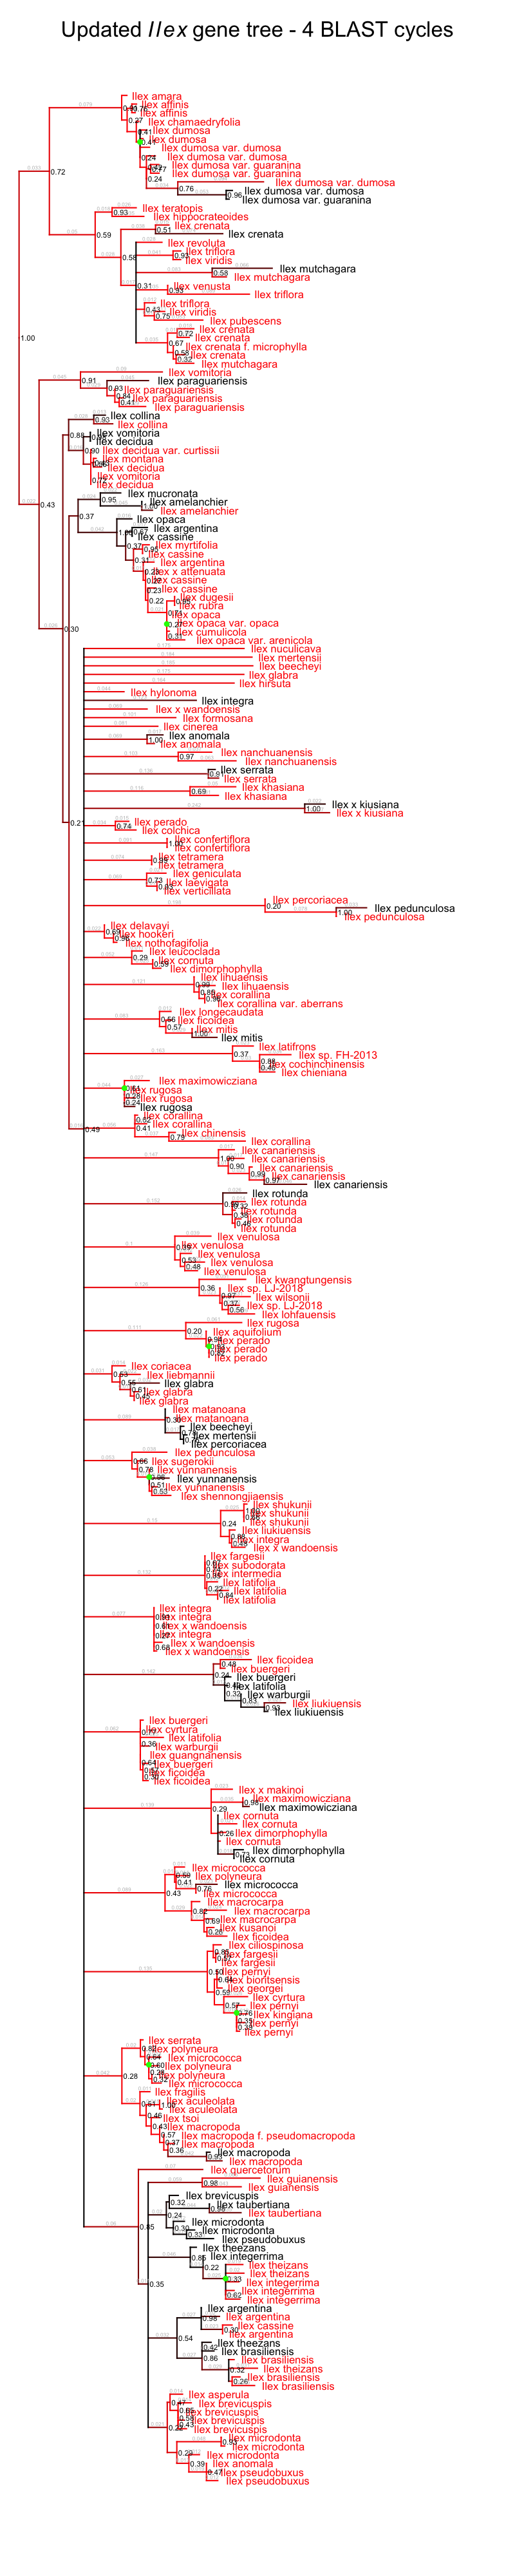
\includegraphics[width=1\linewidth]{docs/figs/ilex-plot-tips-and-branches-1} \caption{A phylogenetic tree is the main result of a Physcraper analysis. In this example, Physcraper updated an alignment of 48 samples of the genus Ilex from Gottlieb et al. 2005 (black tips) and added 222 new samples from the GenBank database (red tips), corresponding to 78 new taxa, aligned the new seqeunces to the original alignment using MUSCLE and performed the phylogenetic reconstruction using RAxML.}\label{fig:ilex-updated-tree}
\end{figure}

The Physcraper updated tree has 57 original tips, representing 51 unique OTT taxa, and 222 new tips representing 78 new OTT taxa added to the original tree.

It has THIS many resolved nodes, and THIS MANY nodes with bootsrap values above 95\%

The original tree has THIS MANY resolved nodes

The alignments have THIS MANY columns and THIS AMOUNT of missing data.

DESCRIBE RESULTS: SUMMARY OF NEW TAXA FOUND RELATIVE TO ORIGINAL TREE AND RELATIVE TO OpenTree
RF DISTANCE INTERPRETATION
HOW MUCH TIME THE BLAST RUN TOOK
ML ESTIMATES OF UPDATED TREE VS ORIGINAL TREE

FIGURE: FACE TO FACE ORIGINAL VS UPDATED PHYLOGENY, IN RED NEW TAXA NOT IN OpenTree.

\hypertarget{the-malvaceae}{%
\subsection{The Malvaceae}\label{the-malvaceae}}

A postdoc started working with a new reserach group. They are interested in solving relationships among lineages of the Malvaceae, a family of flowering plants with almost 6 000 known species, containing the relatives of cacao, cotton, durian and okra.
A review of the literature shows them that there are many phylogenetic trees encompassing some of the linegaes in the group. However, the head of the research group wants to use a particular marker they believe to be the best one to be able to solve the relationships in the group. They have been working on the alignment for a long time and they want to incorporate new data into the hypothesis of homology that they have been curating and that they trust.

\begin{figure}

{\centering 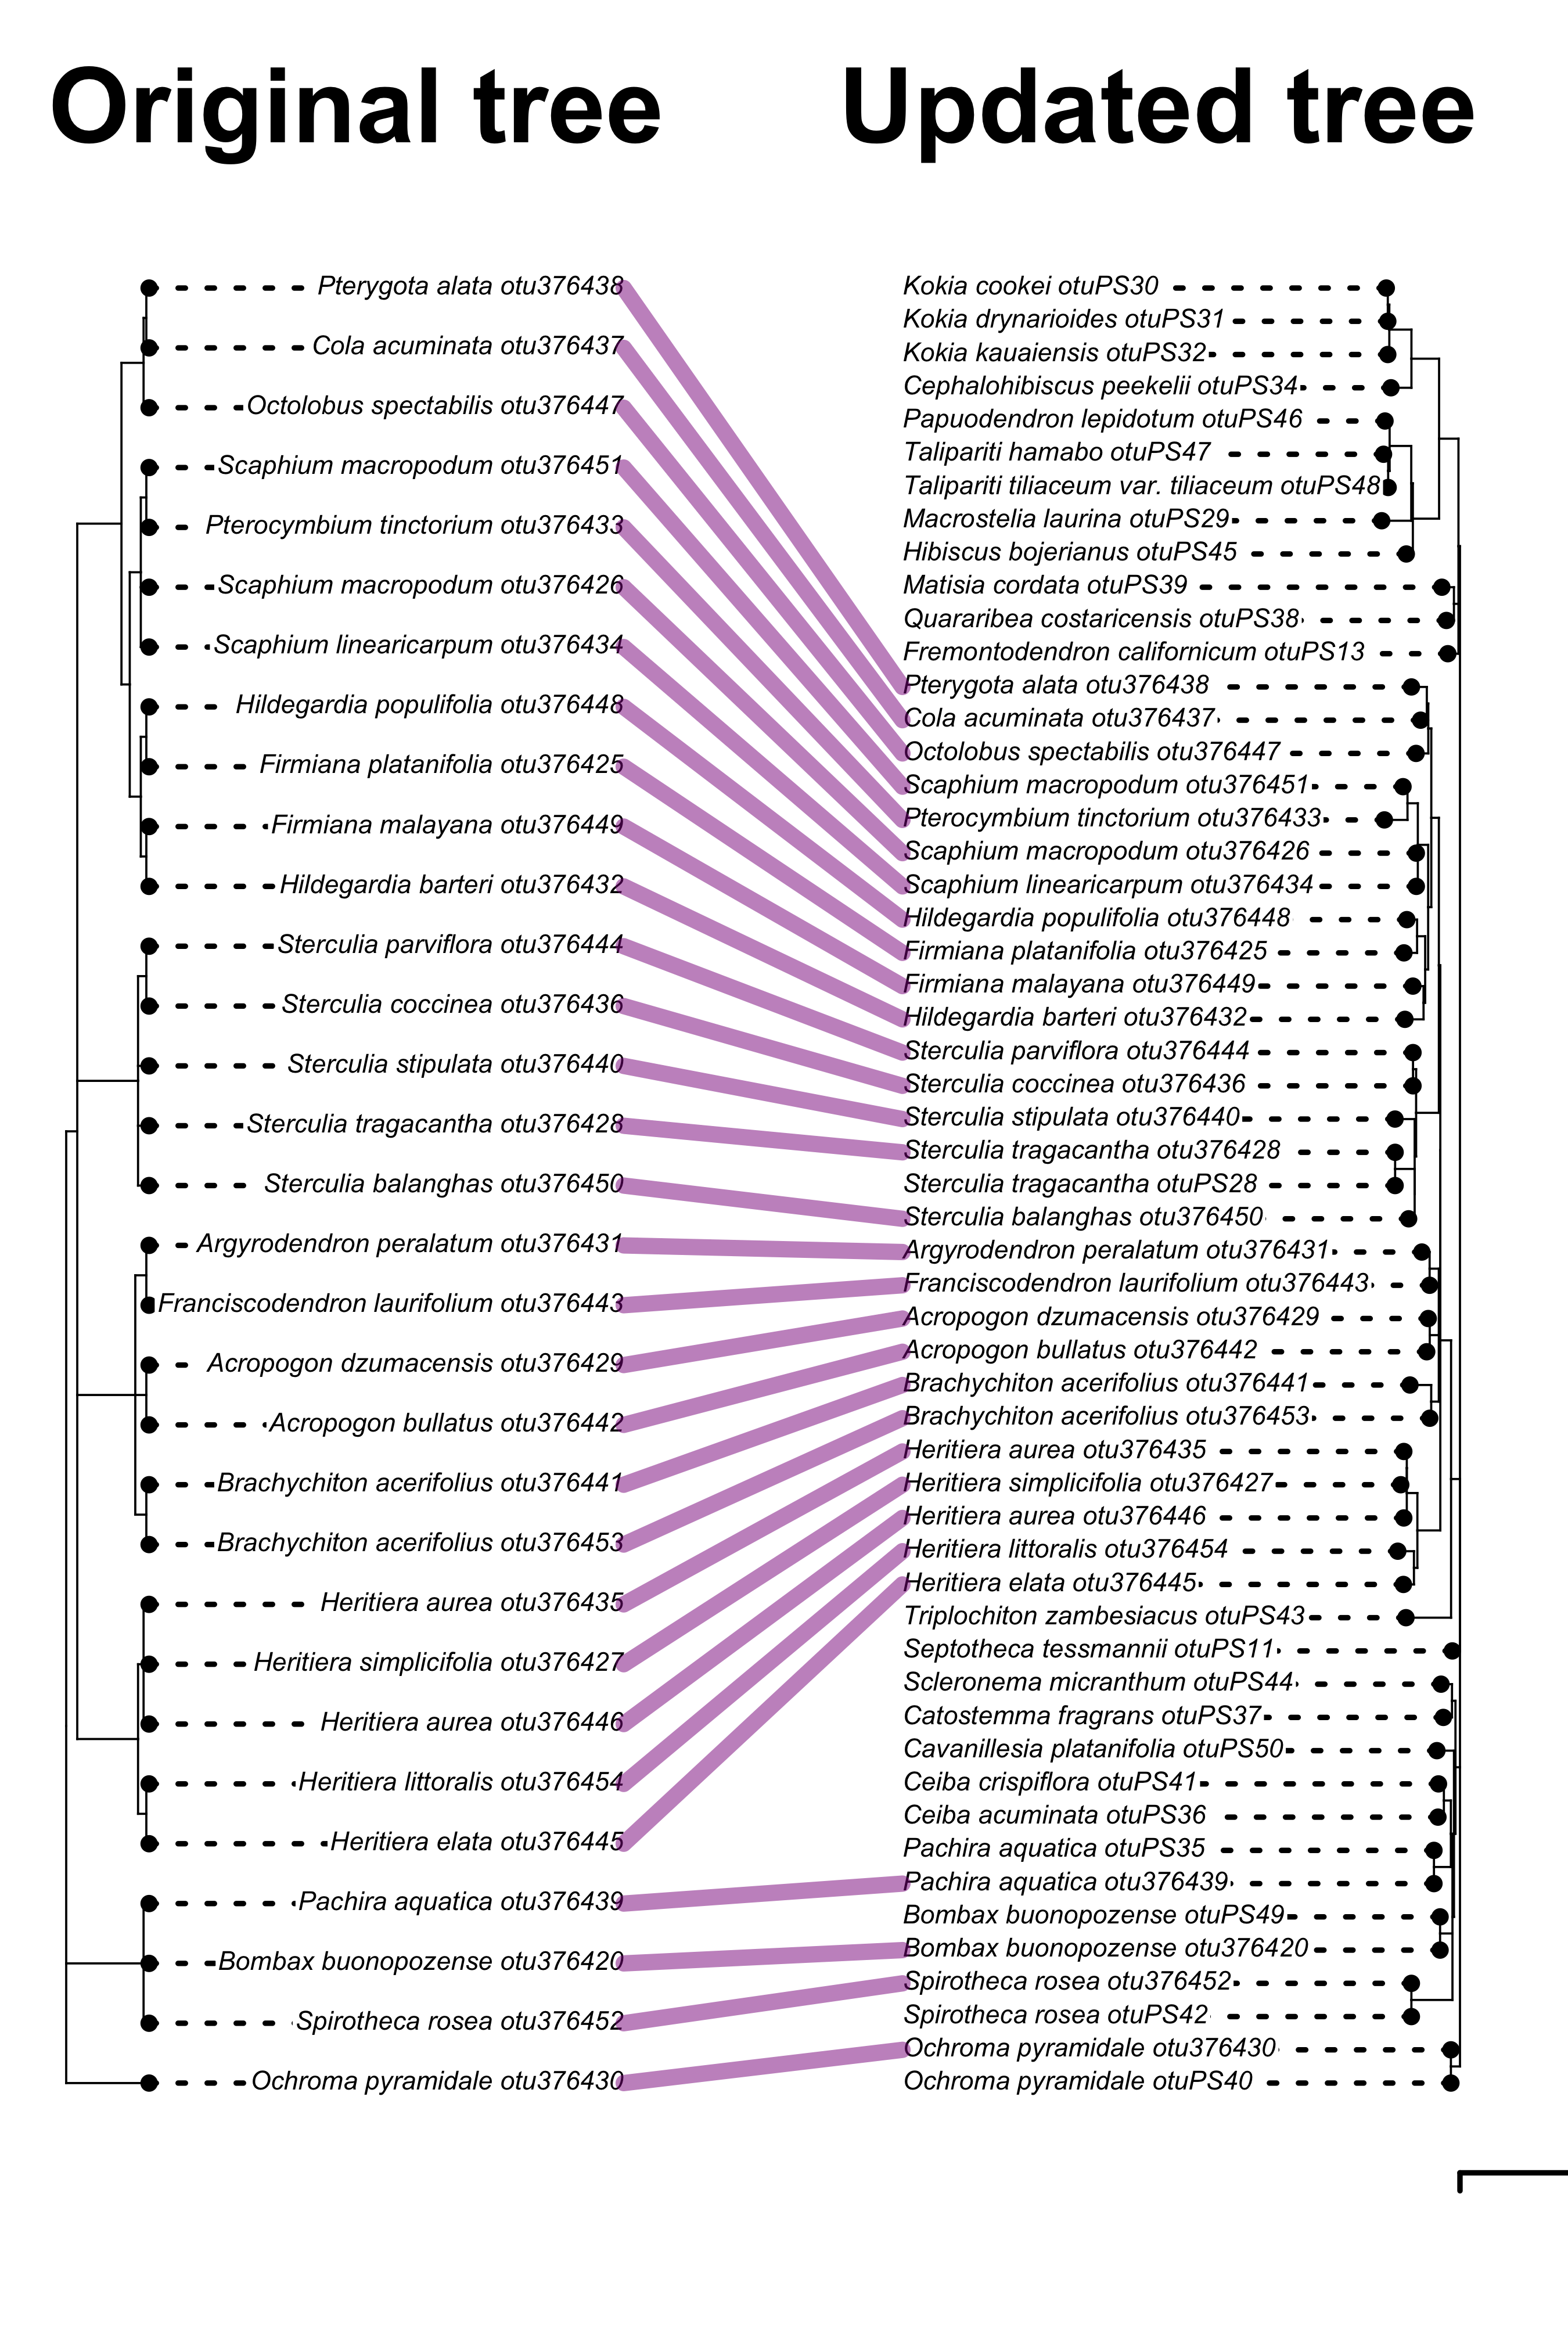
\includegraphics[width=0.85\linewidth]{docs/figs/cotree-plot2-1} 

}

\caption{Comparison of original tree and tree updated with Physcraper, family Malvaceae.}\label{fig:malvaceae}
\end{figure}
\newpage

\hypertarget{discussion}{%
\section{Discussion}\label{discussion}}

Data repositories hold even more information than meets the eye.
Besides the actual data, they are rich sources of metadata that can be used for the advantage of all areas of biology as well as the advancement of scientific policy and applications.

COMPARE WITH PERFORMANCE OF OTHER PIPELINES FOR SEQUENCE SCRAPING
WHY WE DID NOT MAKE A BENCHMARK COMPARISON

Many pipelines are making use of DNA data repositories in different ways.
Most of them focus on efficient ways to mine the data -- getting the most homologs.
Some focus on accurate ways of mining the data -- getting real and clean homologs.
Others focus on refining the alignment.
Most focus on generating full trees \emph{de novo}, mainly for regions of the Tree of
Life that have no phylogenetic assessment yet in published studies, but also for
regions that have already been studied and which have phylogenetic data.
However, expert phylogenetic knowledge is also an important source of data in public
and open repositories that is not being used to its full potential.

All these tools are key efforts for advancing towards reproducibility in phylogenetics,
a field that has relied on processes which are somewhat artisanal.
Here, we highlight the potential of taking advantage of this careful curation work in previous phylogenetic estimates. By taking sources of information available from data repositories and present a method to link data from different repositories, while leveraging the knowledge and intuition of the expert
community to build up our phylogenetic knowledge, we can use not only data accumulated in
molecular data repositories, but phylogenetic knowledge accumulated in phylogenetic tree repositories.

While not generating full phylogenies \emph{de novo}, Physcraper is still capable of generating new phylogenetic knowledge.
Moreover, it can combine phylogenies with data from repositories other than molecular data. For example geographic locations (using GBIF ids), fossils (using PBDB ids), etc. \emph{from Robert: I think you can sell the program more here. Why is it better than the other methods? You mentioned in lab meeting that its difficult to run other programs, talk about that here, talk about the speed and other advantages}

Physcraper has the potential to be applied for the advantage of the field to rapidly \emph{HOW FAST IS ``RAPID'' mention it in results and then here again}
place newly discovered species phylogenetically (Webb \emph{et al.} \protect\hyperlink{ref-webb2010biodiversity}{2010}),
obtain trees for ecophylogenetic studies (Helmus \& Ives \protect\hyperlink{ref-helmus2012phylogenetic}{2012}),
help to systematize molecular databases, i.e., curate taxonomic assignations (San Mauro \& Agorreta \protect\hyperlink{ref-san2010molecular}{2010}),
and rapidly generate custom species trees for downstream analyses (Stoltzfus \emph{et al.} \protect\hyperlink{ref-stoltzfus2013phylotastic}{2013}).

\hypertarget{acknowledgements}{%
\section{Acknowledgements}\label{acknowledgements}}

Research was supported by the grant ``Sustaining the Open Tree of Life'', National Science Foundation ABI No.~1759838, and ABI No.~1759846.
Computer time was provided by the Multi-Environment Research Computer for Exploration and Discovery (MERCED) cluster from the University of California, Merced (UCM), supported by the NSF Grant No.~ACI-1429783.

We thank members of the ``short bar'' Science and Engineering Building 1, University of California Merced, joint lab paper discussion meeting for valuable comments on a first version of this manuscript.

\hypertarget{authors-contributions}{%
\section{Authors' Contributions}\label{authors-contributions}}

EJM: Conceived study, wrote most of the code, documentation and tests.
MK: Wrote code for ncbidataparser module, filtering of sequences per OTU and using offline blast searches, wrote documentation and tests.
LLSR: Wrote the manuscript, alignment code, documentation, performed analyses and developed examples.
All authors contributed to the manuscript.

\hypertarget{data-avilability}{%
\section{Data Avilability}\label{data-avilability}}

Physcraper source code available at \url{https://github.com/McTavishLab/physcraper}
Documentation available at \url{https://physcraper.readthedocs.io/en/latest/index.html}
Illustrated examples available at \url{https://github.com/McTavishLab/physcraperex}
This is a reproducible manuscript available at \url{https://github.com/McTavishLab/physcraper_ms}

\newpage

\hypertarget{references}{%
\section{References}\label{references}}

\newpage
\begin{center}
\textsc{References}
\end{center}

\hypertarget{refs}{}
\leavevmode\hypertarget{ref-altschul1990basic}{}%
Altschul, S.F., Gish, W., Miller, W., Myers, E.W. \& Lipman, D.J. (1990). Basic local alignment search tool. \emph{Journal of molecular biology}, \textbf{215}, 403--410.

\leavevmode\hypertarget{ref-altschul1997gapped}{}%
Altschul, S.F., Madden, T.L., Schäffer, A.A., Zhang, J., Zhang, Z., Miller, W. \& Lipman, D.J. (1997). Gapped blast and psi-blast: A new generation of protein database search programs. \emph{Nucleic acids research}, \textbf{25}, 3389--3402.

\leavevmode\hypertarget{ref-andermann2020guide}{}%
Andermann, T., Torres Jiménez, M.F., Matos-Maraví, P., Batista, R., Blanco-Pastor, J.L., Gustafsson, A.L.S., Kistler, L., Liberal, I.M., Oxelman, B., Bacon, C.D. \& Antonelli, A. (2020). A Guide to Carrying Out a Phylogenomic Target Sequence Capture Project. \emph{Frontiers in Genetics}, \textbf{10}. Retrieved July 28, 2020, from \url{https://www.ncbi.nlm.nih.gov/pmc/articles/PMC7047930/}

\leavevmode\hypertarget{ref-antonelli2017toward}{}%
Antonelli, A., Hettling, H., Condamine, F.L., Vos, K., Nilsson, R.H., Sanderson, M.J., Sauquet, H., Scharn, R., Silvestro, D., Töpel, M. \& others. (2017). Toward a self-updating platform for estimating rates of speciation and migration, ages, and relationships of taxa. \emph{Systematic Biology}, \textbf{66}, 152--166.

\leavevmode\hypertarget{ref-benson2000genbank}{}%
Benson, D.A., Karsch-Mizrachi, I., Lipman, D.J., Ostell, J., Rapp, B.A. \& Wheeler, D.L. (2000). GenBank. \emph{Nucleic acids research}, \textbf{28}, 15--18.

\leavevmode\hypertarget{ref-camacho2009blast}{}%
Camacho, C., George, C., Vahram, A., Ning, M., Jason, P., Kevin, B. \& Thomas, L. (2009). BLAST+: Architecture and applications. \emph{BMC bioinformatics}, \textbf{10}, 421.

\leavevmode\hypertarget{ref-castresana2002gblocks}{}%
Castresana, J. (2002). GBLOCKS: Selection of conserved blocks from multiple alignments for their use in phylogenetic analysis. \emph{Version 0.91 b. Copyrighted by J. Castresana, EMBL}.

\leavevmode\hypertarget{ref-castresana2000selection}{}%
Castresana, J. (2000). Selection of conserved blocks from multiple alignments for their use in phylogenetic analysis. \emph{Molecular biology and evolution}, \textbf{17}, 540--552.

\leavevmode\hypertarget{ref-cock2009biopython}{}%
Cock, P.J., Antao, T., Chang, J.T., Chapman, B.A., Cox, C.J., Dalke, A., Friedberg, I., Hamelryck, T., Kauff, F., Wilczynski, B. \& others. (2009). Biopython: Freely available python tools for computational molecular biology and bioinformatics. \emph{Bioinformatics}, \textbf{25}, 1422--1423.

\leavevmode\hypertarget{ref-cuenoud2000molecular}{}%
Cuénoud, P., Martinez, M.A. del P., Loizeay, P.-A., Spichiger, R., Andrews, S. \& Manen, J.-F. (2000). Molecular phylogeny and biogeography of the genus ilex l.(Aquifoliaceae). \emph{Annals of Botany}, \textbf{85}, 111--122.

\leavevmode\hypertarget{ref-edgar2004muscle}{}%
Edgar, R.C. (2004). MUSCLE: Multiple sequence alignment with high accuracy and high throughput. \emph{Nucleic acids research}, \textbf{32}, 1792--1797.

\leavevmode\hypertarget{ref-fragoso2017pilot}{}%
Fragoso-Martínez, I., Salazar, G.A., Martínez-Gordillo, M., Magallón, S., Sánchez-Reyes, L., Lemmon, E.M., Lemmon, A.R., Sazatornil, F. \& Mendoza, C.G. (2017). A pilot study applying the plant anchored hybrid enrichment method to new world sages (salvia subgenus calosphace; lamiaceae). \emph{Molecular Phylogenetics and Evolution}, \textbf{117}, 124--134.

\leavevmode\hypertarget{ref-gottlieb2005molecular}{}%
Gottlieb, A.M., Giberti, G.C. \& Poggio, L. (2005). Molecular analyses of the genus ilex (aquifoliaceae) in southern south america, evidence from aflp and its sequence data. \emph{American Journal of Botany}, \textbf{92}, 352--369.

\leavevmode\hypertarget{ref-helmus2012phylogenetic}{}%
Helmus, M.R. \& Ives, A.R. (2012). Phylogenetic diversity--area curves. \emph{Ecology}, \textbf{93}, S31--S43.

\leavevmode\hypertarget{ref-izquierdo2014pumper}{}%
Izquierdo-Carrasco, F., Cazes, J., Smith, S.A. \& Stamatakis, A. (2014). PUmPER: Phylogenies updated perpetually. \emph{Bioinformatics}, \textbf{30}, 1476--1477.

\leavevmode\hypertarget{ref-jones2016targeted}{}%
Jones, M.R. \& Good, J.M. (2016). TARGETED CAPTURE IN EVOLUTIONARY AND ECOLOGICAL GENOMICS. \emph{Molecular ecology}, \textbf{25}, 185--202. Retrieved July 28, 2020, from \url{https://www.ncbi.nlm.nih.gov/pmc/articles/PMC4823023/}

\leavevmode\hypertarget{ref-manen2010history}{}%
Manen, J.-F., Barriera, G., Loizeau, P.-A. \& Naciri, Y. (2010). The history of extant ilex species (aquifoliaceae): Evidence of hybridization within a miocene radiation. \emph{Molecular Phylogenetics and Evolution}, \textbf{57}, 961--977.

\leavevmode\hypertarget{ref-mctavish2015phylesystem}{}%
McTavish, E.J., Hinchliff, C.E., Allman, J.F., Brown, J.W., Cranston, K.A., Holder, M.T., Rees, J.A. \& Smith, S.A. (2015). Phylesystem: A git-based data store for community-curated phylogenetic estimates. \emph{Bioinformatics}, \textbf{31}, 2794--2800.

\leavevmode\hypertarget{ref-morrison2006multiple}{}%
Morrison, D.A. (2006). Multiple sequence alignment for phylogenetic purposes. \emph{Australian Systematic Botany}, \textbf{19}, 479--539.

\leavevmode\hypertarget{ref-piel2009treebase}{}%
Piel, W., Chan, L., Dominus, M., Ruan, J., Vos, R. \& Tannen, V. (2009). Treebase v. 2: A database of phylogenetic knowledge. E-biosphere.

\leavevmode\hypertarget{ref-redelings2017supertree}{}%
Redelings, B.D. \& Holder, M.T. (2017). A supertree pipeline for summarizing phylogenetic and taxonomic information for millions of species. \emph{PeerJ}, \textbf{5}, e3058.

\leavevmode\hypertarget{ref-rees2017automated}{}%
Rees, J.A. \& Cranston, K. (2017). Automated assembly of a reference taxonomy for phylogenetic data synthesis. \emph{Biodiversity Data Journal}.

\leavevmode\hypertarget{ref-sanderson2008phylota}{}%
Sanderson, M.J., Boss, D., Chen, D., Cranston, K.A. \& Wehe, A. (2008). The PhyLoTA Browser: Processing GenBank for Molecular Phylogenetics Research. \emph{Systematic Biology}, \textbf{57}, 335--346.

\leavevmode\hypertarget{ref-san2010molecular}{}%
San Mauro, D. \& Agorreta, A. (2010). Molecular systematics: A synthesis of the common methods and the state of knowledge. \emph{Cellular \& Molecular Biology Letters}, \textbf{15}, 311.

\leavevmode\hypertarget{ref-secretariat2017gbif}{}%
Secretariat, G. (2017). GBIF backbone taxonomy. \emph{Checklist Dataset {[}cited 2017 Nov 14{]}. doi}, \textbf{10}.

\leavevmode\hypertarget{ref-selbach2009new}{}%
Selbach-Schnadelbach, A., Cavalli, S.S., Manen, J.-F., Coelho, G.C. \& De Souza-Chies, T.T. (2009). New information for ilex phylogenetics based on the plastid psbA-trnH intergenic spacer (aquifoliaceae). \emph{Botanical Journal of the Linnean Society}, \textbf{159}, 182--193.

\leavevmode\hypertarget{ref-setoguchi2000intersectional}{}%
Setoguchi, H. \& Watanabe, I. (2000). Intersectional gene flow between insular endemics of ilex (aquifoliaceae) on the bonin islands and the ryukyu islands. \emph{American Journal of Botany}, \textbf{87}, 793--810.

\leavevmode\hypertarget{ref-smith2009mega}{}%
Smith, S.A., Beaulieu, J.M. \& Donoghue, M.J. (2009). Mega-phylogeny approach for comparative biology: An alternative to supertree and supermatrix approaches. \emph{BMC evolutionary biology}, \textbf{9}, 37.

\leavevmode\hypertarget{ref-song2012resolving}{}%
Song, S., Liu, L., Edwards, S.V. \& Wu, S. (2012). Resolving conflict in eutherian mammal phylogeny using phylogenomics and the multispecies coalescent model. \emph{Proceedings of the National Academy of Sciences}, \textbf{109}, 14942--14947.

\leavevmode\hypertarget{ref-stamatakis2014raxml}{}%
Stamatakis, A. (2014). RAxML version 8: A tool for phylogenetic analysis and post-analysis of large phylogenies. \emph{Bioinformatics}, \textbf{30}, 1312--1313.

\leavevmode\hypertarget{ref-stoltzfus2013phylotastic}{}%
Stoltzfus, A., Lapp, H., Matasci, N., Deus, H., Sidlauskas, B., Zmasek, C.M., Vaidya, G., Pontelli, E., Cranston, K., Vos, R. \& others. (2013). Phylotastic! Making tree-of-life knowledge accessible, reusable and convenient. \emph{BMC bioinformatics}, \textbf{14}, 158.

\leavevmode\hypertarget{ref-sukumaran2010dendropy}{}%
Sukumaran, J. \& Holder, M.T. (2010). DendroPy: A python library for phylogenetic computing. \emph{Bioinformatics}, \textbf{26}, 1569--1571.

\leavevmode\hypertarget{ref-vos2012nexml}{}%
Vos, R.A., Balhoff, J.P., Caravas, J.A., Holder, M.T., Lapp, H., Maddison, W.P., Midford, P.E., Priyam, A., Sukumaran, J., Xia, X. \& others. (2012). NeXML: Rich, extensible, and verifiable representation of comparative data and metadata. \emph{Systematic biology}, \textbf{61}, 675--689.

\leavevmode\hypertarget{ref-webb2010biodiversity}{}%
Webb, C.O., Slik, J.F. \& Triono, T. (2010). Biodiversity inventory and informatics in southeast asia. \emph{Biodiversity and Conservation}, \textbf{19}, 955--972.

\leavevmode\hypertarget{ref-wheeler2000database}{}%
Wheeler, D.L., Chappey, C., Lash, A.E., Leipe, D.D., Madden, T.L., Schuler, G.D., Tatusova, T.A. \& Rapp, B.A. (2000). Database resources of the national center for biotechnology information. \emph{Nucleic acids research}, \textbf{28}, 10--14.

\leavevmode\hypertarget{ref-yao2020phylogeny}{}%
Yao, X., Song, Y., Yang, J.-B., Tan, Y.-H. \& Corlett, R.T. (2020). Phylogeny and biogeography of the hollies (ilex l., aquifoliaceae). \emph{Journal of Systematics and Evolution}.

\end{document}
